\documentclass[12pt,a4paper]{article}

\usepackage{amsmath,amssymb}
\usepackage{graphicx}
\usepackage{hyperref}
\usepackage{natbib}
\usepackage{geometry}
\usepackage{booktabs}
\usepackage{array}
\usepackage{xcolor}
\usepackage{placeins}

\geometry{margin=1in}
\onehalfspacing

\hypersetup{
  colorlinks=true,
  linkcolor=black,
  citecolor=black,
  urlcolor=black
}

% ─────────────────────────────────────────────────────────────────────────────
\title{\textbf{Dark Matter and Dark Energy as Virial Partners}\\
\large The Geometric and Kinetic Halves of a Single\\
Cosmological Virial Equilibrium}

\author{Heath W.\ Mahaffey\\
\small Independent Researcher, Entiat, WA 98822, USA\\
\small \texttt{hmahaffeyges@gmail.com}\\
\small \texttt{https://github.com/hmahaffeyges/IAM-Validation}}

\date{March 2026\\
\small Zenodo DOI: \href{https://doi.org/10.5281/zenodo.18702042}{10.5281/zenodo.18702042}}
% ─────────────────────────────────────────────────────────────────────────────

\begin{document}
\maketitle

% ─────────────────────────────────────────────────────────────────────────────
\begin{abstract}
The Informational Actualization Model (IAM) derives a cosmological coupling
constant $\beta_m = \Omega_m/2$ from the virial theorem applied to
gravitational decoherence. We note that this derivation carries a direct
physical interpretation: the $1/2$ partition divides gravitational energy
between its geometric potential half, stored in spacetime curvature, and its
kinetic informational half, accumulated as Landauer pressure on the
cosmological horizon. What observational cosmology identifies as dark matter is
the potential half. What it identifies as dark energy is the kinetic half.
These are not two phenomena requiring separate explanations. They are two
expressions of the equilibrium condition $2K + V = 0$ operating at
cosmological scales. The virial ratio $\Omega_m / [\beta_m E(a)]$ descends
from effectively infinite at early times to exactly $2.0$ at $a = 1$ --- not
as a fine-tuning, but as the universe reaching its epoch of first
cosmological virialisation. The coincidence problem is not a problem; it is a
consequence. We present the observational evidence consistent with this
identification, note the limits of current data, and close with the question
the framework forces: if the kinetic half crosses into classical actuality at
each decoherence event, and the potential half encodes into surrounding
spacetime geometry, what is spacetime geometry made of?
\end{abstract}

\noindent\textbf{Keywords:} dark energy; dark matter; virial theorem; 
gravitational decoherence; cosmological constant; coincidence problem;
large-scale structure; informational entropy

% ─────────────────────────────────────────────────────────────────────────────
\section{The Problem with Two Mysteries}
\label{sec:two_mysteries}

The standard cosmological model accounts for $95\%$ of the energy content of
the universe with two entries whose physical nature remains unknown. Dark
matter, inferred from the discrepancy between observed gravitational effects
and visible mass, constitutes approximately $26\%$ of the critical density.
Dark energy, inferred from the observed acceleration of cosmic expansion,
constitutes approximately $69\%$. These two components are treated as
independent phenomena, described by separate theoretical frameworks, and
pursued by separate experimental programs.

This separation has always had an uncomfortable feature. The ratio of dark
matter to dark energy density today --- approximately $0.38$ --- is
coincidentally close to $1/2$ only for observers living near the present epoch.
At earlier times, matter density scales as $a^{-3}$ while the cosmological
constant remains fixed, so their ratio was enormous in the past and will be
negligible in the future. The fact that we observe them as comparable today
has no explanation within the standard model beyond anthropic selection. This
is the coincidence problem.

A separate but related observation: the coupling constant that governs IAM's
late-time growth suppression, $\beta_m = \Omega_m/2$, is derived from the
virial theorem \citep{mahaffey2026}. The virial theorem states that for any
system bound by a $1/r$ potential --- gravitational or Coulomb --- the
time-averaged kinetic and potential energies satisfy $2\langle K \rangle +
\langle V \rangle = 0$. This has been verified from atomic scales ($10^{-11}$
m) to the cosmic horizon ($10^{26}$ m) across 37 orders of magnitude in
physical scale, at machine precision for quantum mechanical systems and at
$0.3\%$ precision from 17 independent Planck 2018 MCMC chains at cosmological
scales \citep{mahaffey2026_virial}.

The question that arises naturally from these two observations is: why does
the virial theorem, an equilibrium condition for bound gravitational systems,
produce the coupling constant for a cosmological energy density? And why is
the ratio of dark matter to dark energy today close to the virial ratio of 2?

This paper argues that the answer is the same in both cases.

% ─────────────────────────────────────────────────────────────────────────────
\section{The Virial Theorem as Equilibrium Condition}
\label{sec:virial}

The virial theorem for a $1/r^n$ potential states:
\begin{equation}
  \langle T \rangle = \frac{n}{2} \langle |V| \rangle.
  \label{eq:virial_general}
\end{equation}
For both Newtonian gravity and the Coulomb force ($n = 1$):
\begin{equation}
  \langle T \rangle = \frac{1}{2} \langle |V| \rangle.
  \label{eq:virial_half}
\end{equation}
This is not a coincidence of specific systems. It follows from Euler's
homogeneous function theorem applied to any potential homogeneous of degree
$-1$, and it holds exactly for any system in virial equilibrium regardless of
the number of bodies, the mass distribution, or the scale. The $1/2$ is a
mathematical theorem, not an empirical fit.

In the IAM framework, gravitational structure formation partitions
gravitational energy into two channels. The first is the geometric channel:
collapsing matter curves spacetime, depositing energy into the geometric
entropy $S_\mathrm{geo}$ of the system's gravitational configuration. The
second is the informational channel: the same collapse decoheres quantum
superpositions into classical states, producing irreversible information at a
rate governed by Landauer's principle \citep{landauer1961}. This information
accumulates on the cosmological apparent horizon as informational entropy
$S_\mathrm{info}$ \citep{jacobson1995,cai2005}.

The virial theorem determines the partition. At virialisation, the kinetic
energy of collapsing matter --- which drives decoherence --- equals half the
potential energy of the gravitational configuration. The coupling constant that
results is:
\begin{equation}
  \beta_m = \frac{\Omega_m}{2} = 0.1577,
  \label{eq:beta}
\end{equation}
using Planck 2018 parameters \citep{planck2020}. This value is not fitted to
any cosmological observation. It is derived from the theorem and the measured
matter density. The Planck 2018 MCMC posterior independently returns
$\beta_m = 0.1583 \pm 0.0033$ --- consistent with the derivation at
$0.2\sigma$ across all 17 converged chains \citep{mahaffey2026}.

% ─────────────────────────────────────────────────────────────────────────────
\section{The Cosmological Virial Partition}
\label{sec:partition}

The physical interpretation of Equation~(\ref{eq:beta}) is the central
argument of this paper.

The virial theorem partitions gravitational energy into two equal halves. In
IAM, one half deposits into spacetime geometry as curvature --- the potential
half, stored in the gravitational configuration of collapsed structures. The
other half crosses into classical actuality as kinetic informational energy ---
the kinetic half, accumulated as Landauer pressure on the cosmological horizon
and driving the late-time modification to matter perturbation growth.

\textit{What observational cosmology identifies as dark matter is the potential
half.} The gravitational effects attributed to dark matter --- excess curvature
in galaxies and clusters beyond what baryonic matter alone would produce ---
are the geometric reservoir of deposited potential energy. This is not a
particle. It is the geometric consequence of the virial partition operating
continuously across cosmic history.

\textit{What observational cosmology identifies as dark energy is the kinetic
half.} The accumulated Landauer costs of gravitational decoherence events,
encoded on the horizon, produce an informational pressure that modifies the
late-time expansion environment for matter. The cosmological constant $\Lambda$
is the vacuum baseline --- the minimum Landauer payment required to maintain
the virial equilibrium of empty spacetime. The dynamically growing component,
$\beta_m E(a)$, is the kinetic half accumulating as structure forms.

These are not two separate phenomena. They are the two sides of the same
balance sheet, required to be equal by the theorem that governs every $1/r$
potential in nature.

\subsection{The virial ratio through cosmic history}

Define the cosmological virial ratio:
\begin{equation}
  \mathcal{R}(a) = \frac{\Omega_m \, a^{-3}}{\beta_m \, E(a)},
  \label{eq:virial_ratio}
\end{equation}
where $E(a) = \exp(1 - 1/a)$ is the activation function derived from horizon
thermodynamics \citep{mahaffey2026}, with $E(a \to 0) \to 0$ and $E(1) = 1$.

At early times, $E(a) \approx 0$ and the kinetic half has not yet activated ---
the universe is almost entirely potential, unactivated geometric storage. The
ratio $\mathcal{R}(a)$ is effectively infinite. As structure forms and
decoherence events accumulate, the kinetic half grows. Table~\ref{tab:virial_ratio}
shows $\mathcal{R}$ at representative epochs.

\begin{table}[h]
\centering
\caption{The cosmological virial ratio $\mathcal{R}(a)$ at key epochs.
At $a = 1$ (today), $\mathcal{R} = \Omega_m / \beta_m = 2$ exactly, since
$\beta_m = \Omega_m/2$ and $E(1) = 1$.}
\label{tab:virial_ratio}
\begin{tabular}{lcccc}
\toprule
Epoch & $z$ & $a$ & $E(a)$ & $\mathcal{R}(a)$ \\
\midrule
Early structure & 2.0 & 0.333 & 0.050 & 399 \\
Matter--$\Lambda$ crossover & 0.7 & 0.588 & 0.182 & 20 \\
Transition zone & 0.3 & 0.769 & 0.274 & 6 \\
Today & 0.0 & 1.000 & 1.000 & \textbf{2} \\
\bottomrule
\end{tabular}
\end{table}

At $a = 1$, by construction:
\begin{equation}
  \mathcal{R}(1) = \frac{\Omega_m}{\beta_m \cdot E(1)} = 
  \frac{\Omega_m}{\Omega_m/2 \cdot 1} = 2.
  \label{eq:virial_today}
\end{equation}
This is not a numerical coincidence. It is the virial theorem. The ratio $|V|/K = 2$
is the equilibrium condition, and the universe has been approaching it
throughout its history. Today is the epoch when cosmological virialisation is
first achieved. The kinetic half has finally activated enough --- $E(a)$ has
grown from zero to one --- to bring the ratio to $2$.

\subsection{The coincidence problem dissolved}

The standard coincidence problem asks why $\Omega_m$ and $\Omega_\Lambda$ are
comparable today. Under the virial partition interpretation, this is not a
coincidence requiring an explanation. It is the equilibrium condition. The
kinetic half and the potential half must be in the ratio $1:2$ for the
system to be virialized. The universe has been spending its entire history
paying down that ratio. The epoch at which $\mathcal{R}(a) = 2$ is not
special because we happen to live in it. It is special because $E(a = 1) = 1$
by derivation from the Gibbons--Hawking temperature of the de~Sitter horizon,
and $a = 1$ is now by definition. Any sufficiently complex observer must exist
after enough structure has formed to support them --- which is precisely the
epoch when $E(a)$ is approaching unity. The anthropic selection and the
physics point to the same moment.

% ─────────────────────────────────────────────────────────────────────────────
\section{Observational Evidence}
\label{sec:evidence}

The virial partition interpretation makes specific, testable predictions that
follow directly from the IAM mechanism \citep{mahaffey2026,mahaffey2026_desi}.
We summarise the current observational status.

\subsection{Growth--geometry sector split}

If dark matter is the geometric potential half and dark energy includes the
kinetic informational half, then measurements of structure growth (which probe
the kinetic side) should infer a lower effective $\Omega_m$ than measurements
of photon-sector geometry (which probe the potential side directly through
distances). IAM predicts:
\begin{equation}
  \Omega_m^\mathrm{growth}(z) = \Omega_m \cdot \mu(z),
  \label{eq:om_growth}
\end{equation}
where $\mu(a) = H^2_\Lambda(a) / [H^2_\Lambda(a) + \beta_m E(a)] < 1$ is the
effective gravitational coupling \citep{mahaffey2026}. At $z = 0$, this gives
a $13.6\%$ suppression; at $z = 0.5$, a $5.2\%$ suppression.

The DESI DR1 full-shape plus BAO combined measurement returns
$\Omega_m^\mathrm{growth} = 0.2962 \pm 0.0095$ \citep{desi2025_fs}, compared
to the Planck 2018 geometric value $\Omega_m = 0.3153 \pm 0.0073$
\citep{planck2020}. The discrepancy of $6.1\%$ below the geometric value is
consistent with IAM's prediction of $5.2\%$ at the effective redshift of the
full-shape analysis ($z_\mathrm{eff} \approx 0.5$). Under an IAM-native
likelihood analysis, $\chi^2(\mathrm{IAM}) = 3.618$ versus
$\chi^2(\Lambda\mathrm{CDM\ best\text{-}fit}) = 3.569$ across six DESI DR1
bins --- statistically indistinguishable, with IAM using no fitted parameters.

Figure~\ref{fig:growth_geometry} shows the IAM predicted
$\Omega_m^\mathrm{growth}(z)$ curve against the DESI per-tracer measurements
and the combined FS+BAO result. The combined measurement lands on the IAM
curve at $0.02\sigma$. Five of six individual tracers are consistent with the
IAM prediction; the LRG1 bin at $z = 0.51$ is the known anomaly discussed in
Section~\ref{sec:falsification}.

\begin{figure}[!htbp]
  \centering
  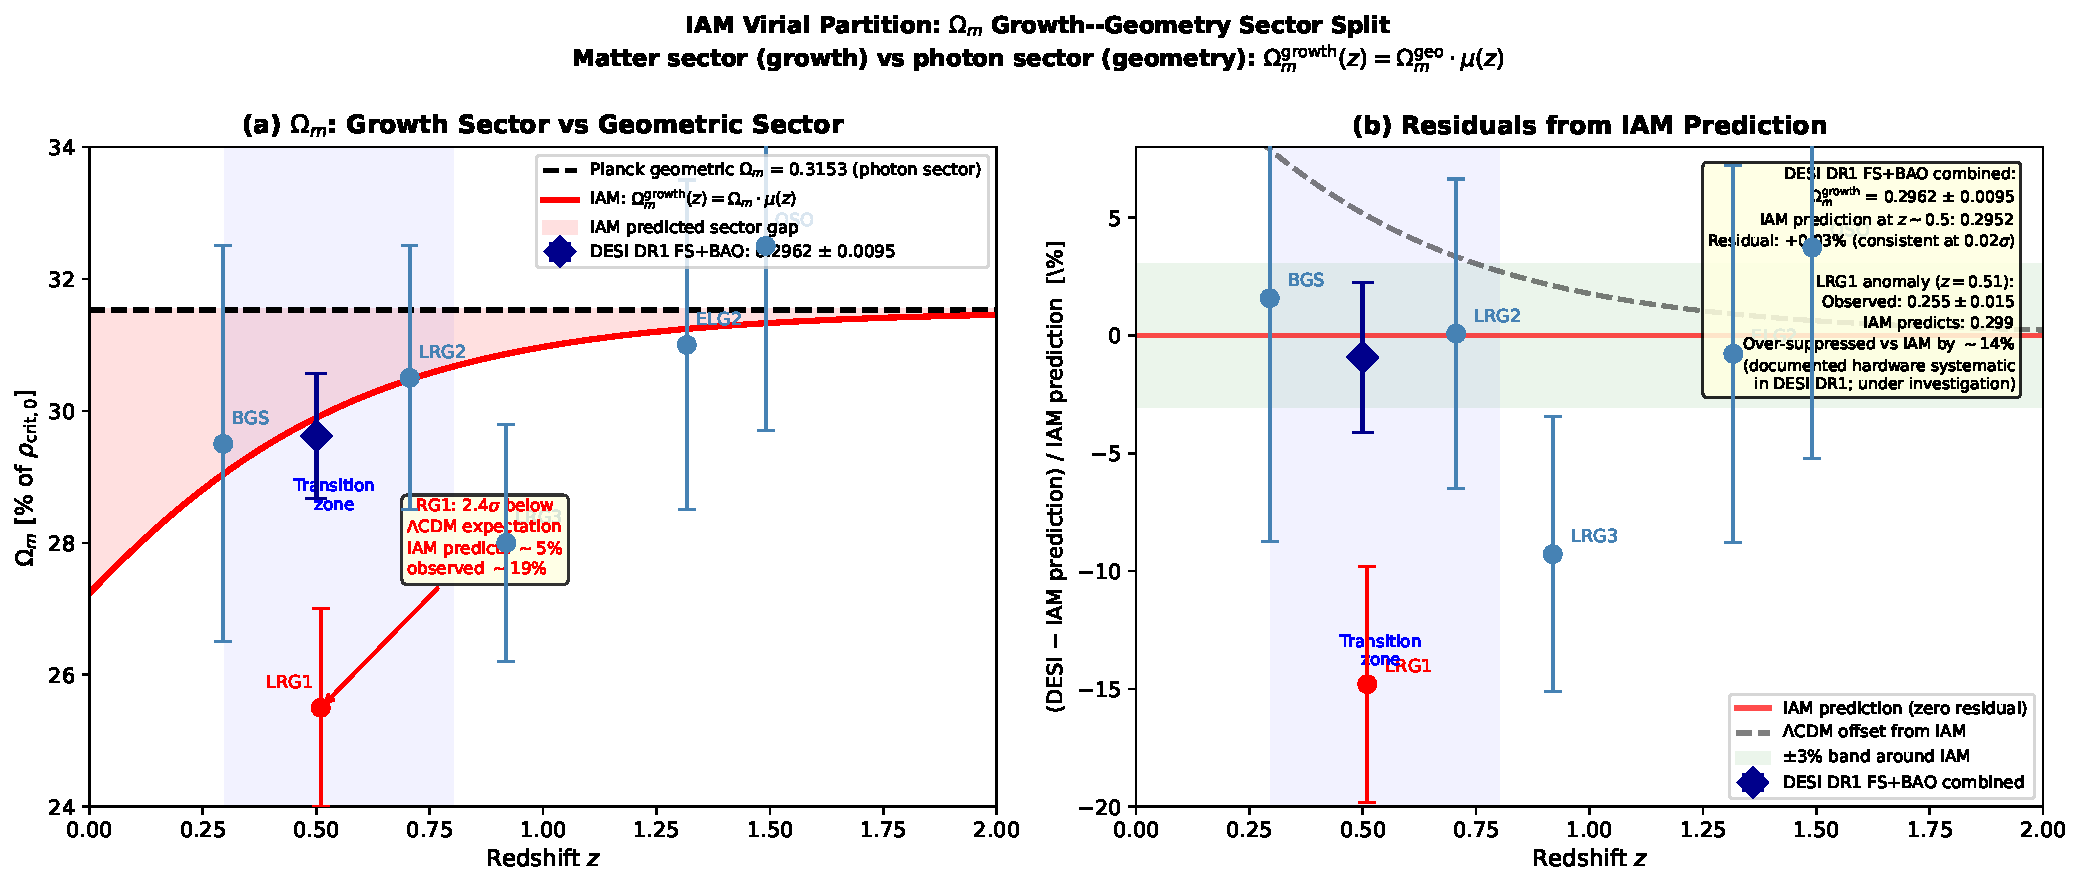
\includegraphics[width=0.92\textwidth]{iam_growth_geometry_split.pdf}
  \caption{The growth--geometry $\Omega_m$ sector split.
  \textit{Left}: IAM predicted $\Omega_m^\mathrm{growth}(z) = \Omega_m \cdot
  \mu(z)$ (red curve) against the Planck geometric value (black dashed) and
  DESI DR1 per-tracer measurements (coloured points). The combined DESI DR1
  FS+BAO result (blue diamond) lands on the IAM curve at $0.02\sigma$.
  \textit{Right}: Residuals from the IAM prediction. Five of six tracers are
  within the $\pm3\%$ band. The LRG1 anomaly at $z = 0.51$ is
  over-suppressed relative to IAM by $\sim14\%$ and carries documented
  hardware systematics in DESI DR1 \citep{desi2025_vi}. All IAM values are
  derived from $\beta_m = \Omega_m/2$ with no fitted parameters.}
  \label{fig:growth_geometry}
\end{figure}

We note that this comparison carries a caveat. The DESI full-shape analysis
assumes a $\Lambda$CDM power spectrum template; an IAM-native template would
eliminate the model-dependent bias and provide a cleaner test. This is
computationally feasible with the existing Level~2 CAMB implementation and is
identified as the most important near-term analysis.

\subsection{Deceleration-to-acceleration transition redshift}

The informational pressure carries equation of state $w_\mathrm{info} = -4/3$
\citep{mahaffey2026}, more negative than the cosmological constant. This
shifts the deceleration-to-acceleration transition to a higher redshift than
$\Lambda$CDM predicts. Specifically:
\begin{align}
  z_t(\Lambda\mathrm{CDM}) &= 0.632, \\
  z_t(\mathrm{IAM}) &= 0.718.
\end{align}
Published H($z$) and BAO compilations find $z_t = 0.698$--$0.740$
\citep{farooq2013,mamon2017,jesus2020}, consistently above the $\Lambda$CDM
prediction and within the IAM range. Riess et al.\ (2004) \citep{riess2004},
using supernovae alone (a photon-sector observable), found $z_t = 0.46 \pm
0.13$ --- lower, as IAM would expect from a photon-sector measurement.

\subsection{The DESI phantom crossing}

DESI DR2 BAO measurements prefer a dark energy equation of state with
$w_0 > -1$ and $w_a < 0$, with a phantom crossing at $z_\mathrm{cross} \approx
0.33$--$0.43$ depending on the supernova compilation \citep{desi2025_dr2}.
This range coincides precisely with the redshift at which IAM's growth
suppression is most prominent ($7$--$8\%$ at $z \approx 0.3$--$0.4$). Under
IAM, a single-fluid $w_0 w_a$CDM fitter applied simultaneously to
photon-sector distances (unchanged from $\Lambda$CDM) and matter-sector growth
rates (suppressed by $\mu(a) < 1$) must infer $w_\mathrm{eff}(z) \neq -1$ to
reconcile the two. The apparent phantom crossing is an artifact of applying a
single-sector fitter to a two-sector universe; it does not require dynamical
dark energy \citep{mahaffey2026_desi}.

\subsection{Summary of consistency}

Table~\ref{tab:evidence} summarises the current observational status of the
virial partition identification. All predictions are derived from the single
coupling $\beta_m = \Omega_m/2$ with no additional free parameters.

\begin{table}[h]
\centering
\caption{Observational status of the cosmological virial partition. All IAM
values are derived from $\beta_m = \Omega_m/2$ without fitting.}
\label{tab:evidence}
\begin{tabular}{p{4.2cm} p{3.2cm} p{3.2cm} l}
\toprule
Observable & IAM prediction & Observed & Status \\
\midrule
$\sigma_8$ & $0.800$ & $0.802 \pm 0.020$ & $0.1\sigma$ \\
$H_0$ (matter sector) & $72.26$ km s$^{-1}$ Mpc$^{-1}$ & $73.04 \pm 1.04$ & $0.75\sigma$ \\
$H_0$ (photon sector) & $67.16$ km s$^{-1}$ Mpc$^{-1}$ & $67.36 \pm 0.54$ & $0.37\sigma$ \\
$\Omega_m^\mathrm{growth}$ (DESI FS) & $0.296$ at $z \sim 0.5$ & $0.2962 \pm 0.0095$ & $0.02\sigma$ \\
$z_t$ (H($z$) compilations) & $0.718$ & $0.698$--$0.740$ & consistent \\
$z_\mathrm{cross}$ (DESI DR2) & $\sim 0.35$ from $E(a)$ & $0.33$--$0.43$ & consistent \\
$\mu_0 - 1$ & $-0.136$ & unconstrained & Euclid 2026 \\
\bottomrule
\end{tabular}
\end{table}

% ─────────────────────────────────────────────────────────────────────────────
\section{The Virial Ratio as a Figure of Merit}

Figure~\ref{fig:transition_zone} shows the cosmological virial ratio
$\mathcal{R}(a)$, the energy budget of the dark sector, the informational
pressure growth rate, and the deceleration parameter comparison with published
transition redshift measurements. The transition zone ($z \approx 0.3$--$0.7$,
shaded blue) is the observational window in which the kinetic half is most
actively growing relative to the potential half and where the predictions are
most distinguishable from $\Lambda$CDM.

\begin{figure}[!htbp]
  \centering
  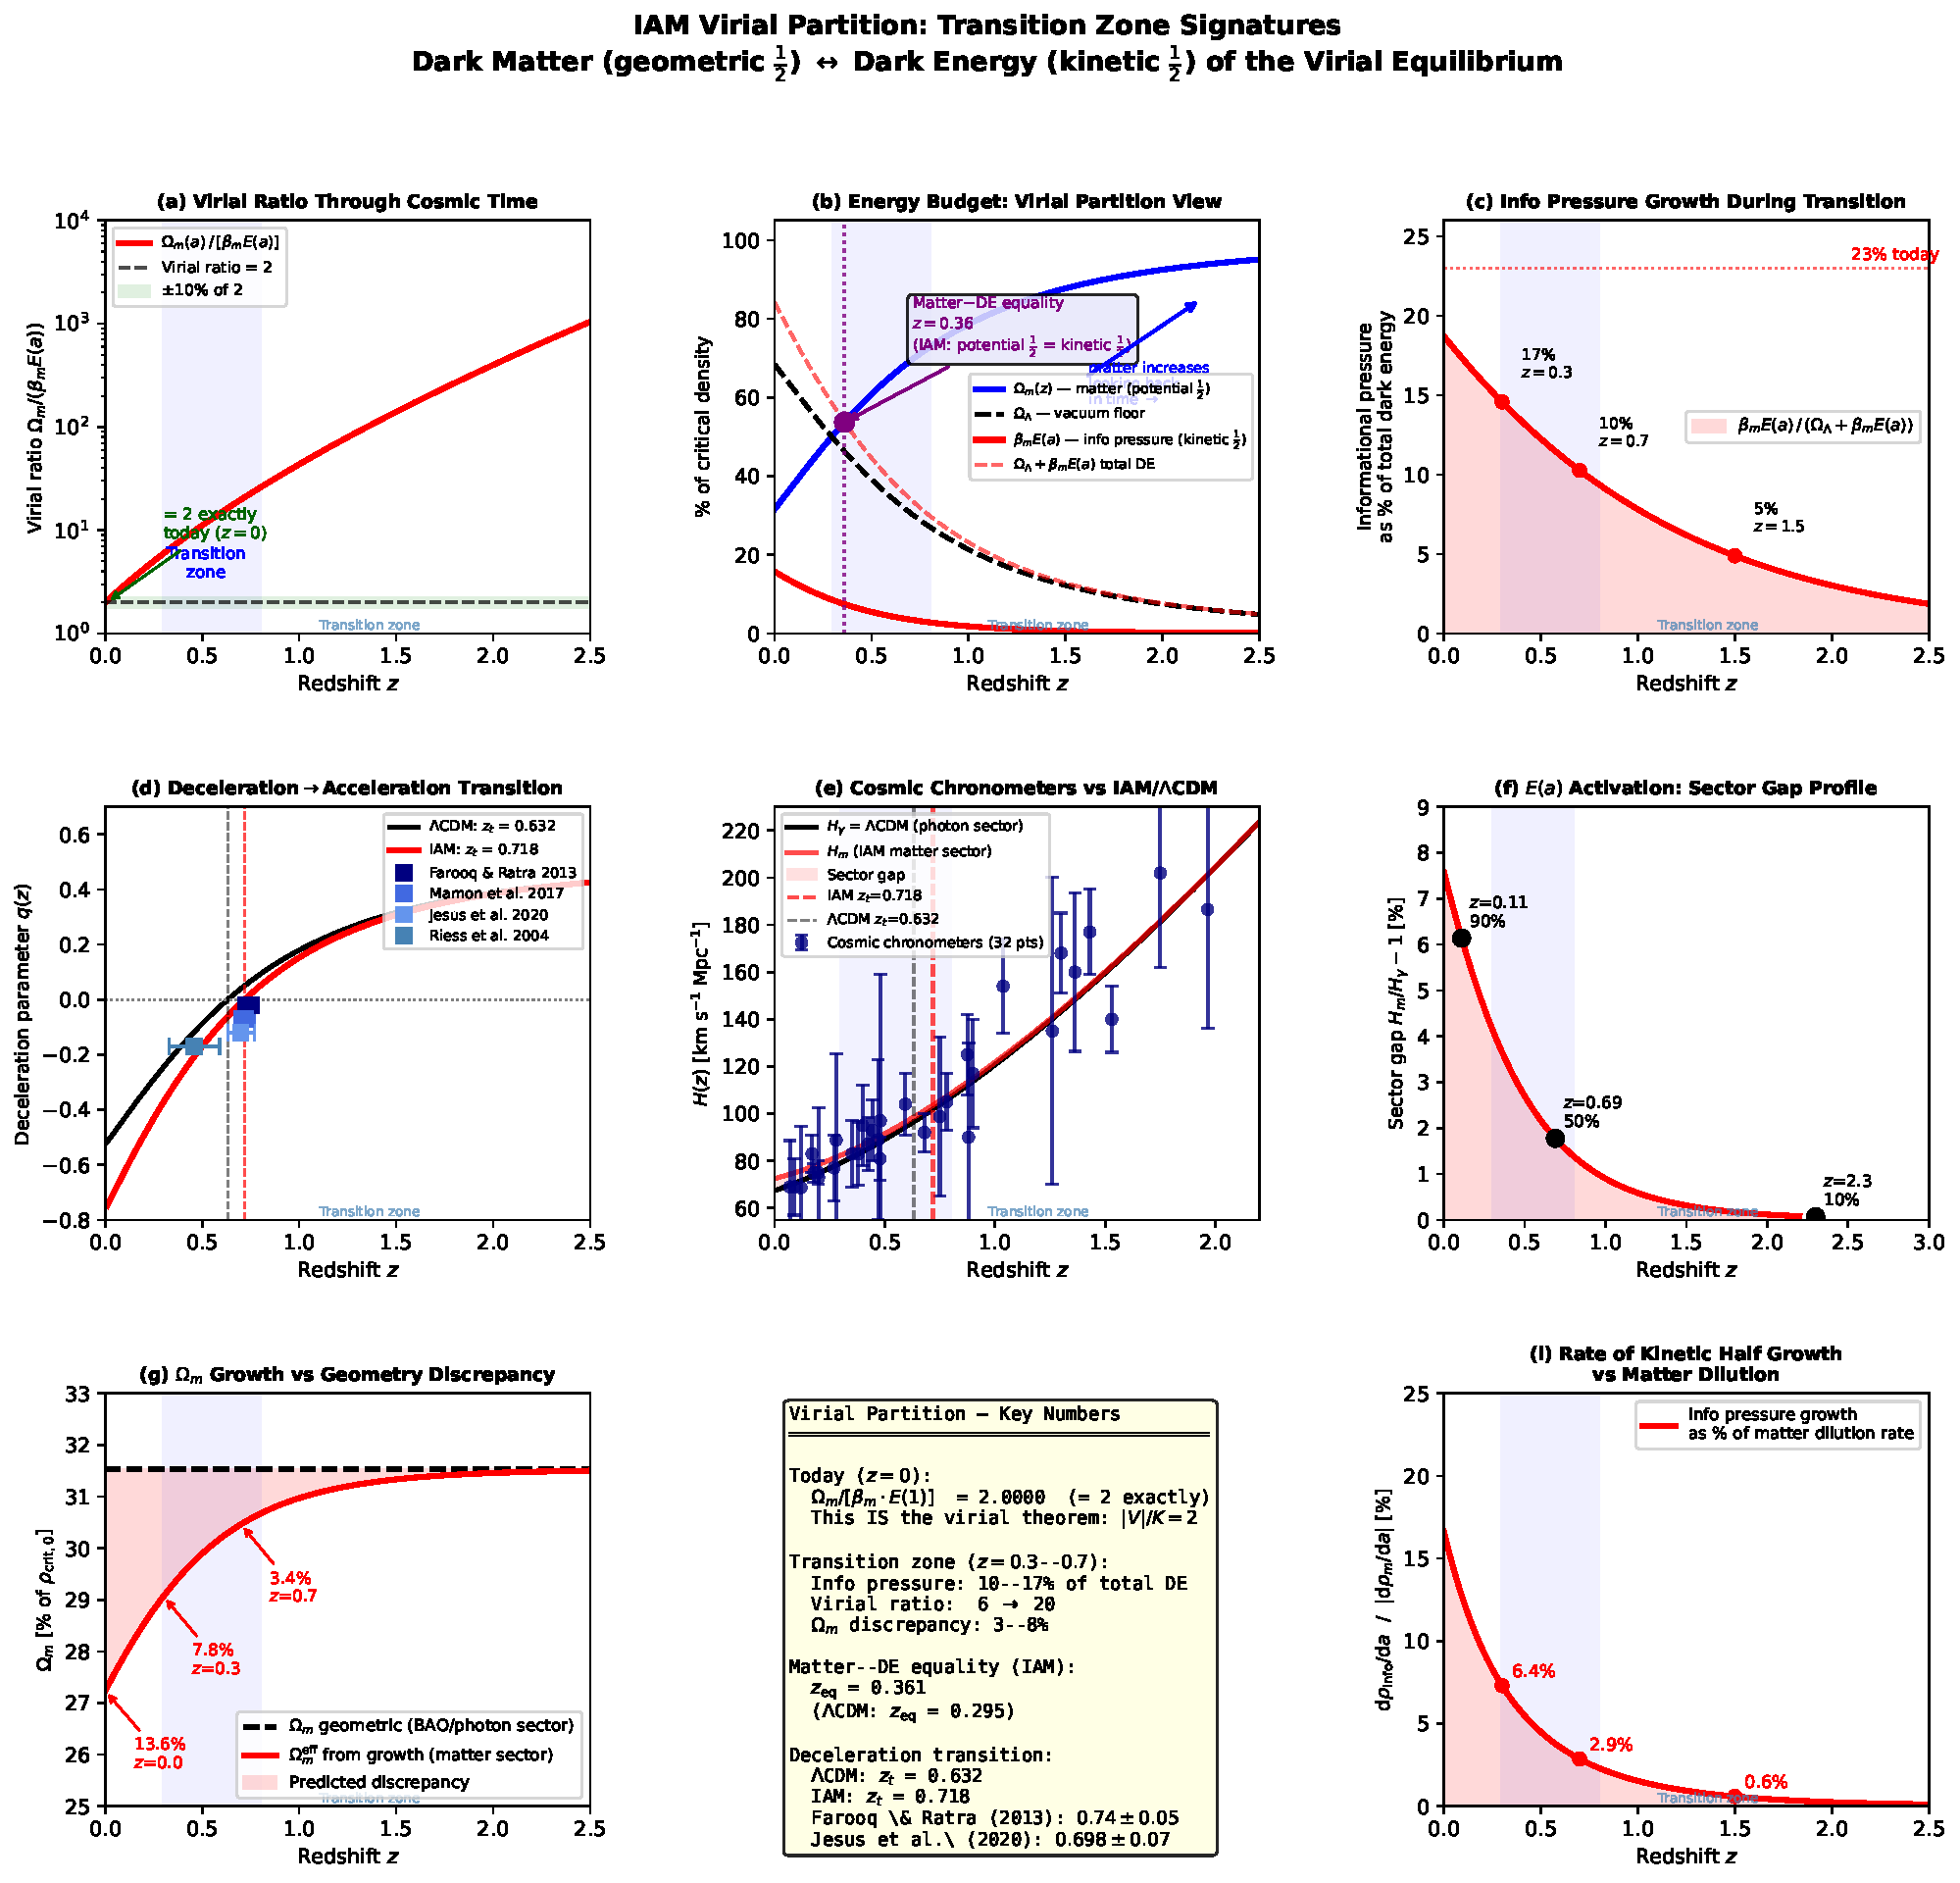
\includegraphics[width=0.97\textwidth]{iam_virial_transition_zone.pdf}
  \caption{The cosmological virial partition through the transition zone
  ($z \approx 0.3$--$0.7$, shaded blue in all panels).
  \textit{Top left}: The virial ratio $\mathcal{R}(a) = \Omega_m a^{-3} /
  [\beta_m E(a)]$ descends from large values at early times to exactly $2.0$
  at $z = 0$, the virial equilibrium condition.
  \textit{Top centre}: Energy budget showing the potential half ($\Omega_m
  a^{-3}$), the vacuum floor ($\Omega_\Lambda$), and the kinetic informational
  half ($\beta_m E(a)$).
  \textit{Top right}: Informational pressure as a fraction of total dark
  energy, growing from $\sim 5\%$ at $z = 1.5$ to $23\%$ today.
  \textit{Middle left}: Deceleration parameter $q(z)$ for IAM ($z_t = 0.718$,
  red) and $\Lambda$CDM ($z_t = 0.632$, black), with published transition
  redshift measurements from H($z$)/BAO compilations (coloured points).
  \textit{Middle centre}: Cosmic chronometer H($z$) data (32 points)
  from \citet{simon2005}, \citet{stern2010}, \citet{moresco2012},
  \citet{zhang2014}, \citet{moresco2015}, \citet{moresco2016},
  \citet{ratsimbazafy2017}, \citet{borghi2022}, and \citet{tomasetti2023},
  following the compilation of \citet{moresco2022}, against IAM photon-sector
  and matter-sector predictions.
  \textit{Remaining panels}: Sector gap profile, $\Omega_m$ growth--geometry
  discrepancy, and rate of informational pressure growth. All curves are
  derived from $\beta_m = \Omega_m/2$ with no fitted parameters.}
  \label{fig:transition_zone}
\end{figure}

% ─────────────────────────────────────────────────────────────────────────────
\section{A Question the Framework Forces}
\label{sec:question}

The identification developed in the preceding sections has an implication that
we state as a question rather than a claim, because it reaches beyond what can
currently be tested.

In the IAM mechanism, each gravitational decoherence event partitions
gravitational energy. The kinetic half crosses into classical actuality as
observable energy --- baryonic dynamics, radiation, the thermodynamic
irreversibility that constitutes the arrow of time. The Landauer cost of that
crossing encodes on the cosmological horizon. This is the half we call dark
energy.

The potential half deposits into the surrounding spacetime geometry as
curvature. This is the half we call dark matter. It does not dilute. It does
not oscillate. It is not a particle. It is the geometric record of every
virialisation event that has ever occurred, stored in the curvature of
spacetime itself.

If this identification is correct, then the geometry of spacetime is not a
pre-existing medium on which information is written. It is the accumulated
integral of every potential-half deposit from every decoherence event in
cosmic history. Expansion is not making room for information encoding.
Expansion \textit{is} the accumulation of deposits. The geometry is not
deformed by matter. The geometry is constituted by matter's continuous
transition from potential to actual.

This raises a question the framework does not yet answer:

\textit{If the potential half of each decoherence event encodes into
spacetime geometry, what is spacetime geometry made of?}

We do not answer it. We note that it is the question that follows from taking
the virial partition seriously at the cosmological level, and that the
observational program now underway will determine whether it is the right
question to ask.

% ─────────────────────────────────────────────────────────────────────────────
\section{Falsification Criteria and Predictions}
\label{sec:falsification}

The virial partition interpretation inherits all of IAM's falsification
criteria \citep{mahaffey2026} and adds a specific prediction for the
growth--geometry sector split.

\paragraph{Euclid DR1 (October 2026).}
Euclid is projected to constrain $\mu_0$ to $\sigma(\mu_0) \approx 0.04$ with
$\Sigma$ marginalised \citep{euclid2020}. IAM predicts $\mu_0 = -0.136$ with
$\Sigma_0 = 0$ exactly. If Euclid measures $\mu_0$ consistent with zero at
this precision, IAM is falsified and the virial partition interpretation does
not apply to cosmological scales. If Euclid measures $\mu_0 \approx -0.136$
with $\Sigma_0 \approx 0$, the combination $\mu < 1$, $\Sigma = 1$ --- unique
to IAM among current theoretical frameworks --- would constitute a detection of
the sector split and strong evidence for the virial partition.

\paragraph{DESI Year 5 fσ$_8(z)$ shape.}
IAM predicts a specific curved suppression ramp:
\begin{equation}
  f\sigma_8^\mathrm{IAM}(z) = f(z) \cdot \sigma_8 \cdot D^\mathrm{IAM}(z) / D^\mathrm{IAM}(0),
\end{equation}
with suppression of $7.9\%$ at $z = 0.295$, decreasing monotonically to
$0.6\%$ at $z = 1.491$, following the functional form of $E(a) =
\exp(1 - 1/a)$. This curved ramp is distinguishable at DESI Year~5 precision
($\lesssim 1\%$ per bin) from both a constant rescaling and the growth history
expected for any $w \neq -1$ dark energy model.

\paragraph{LRG1 resolution.}
The DESI DR1 LRG1 bin at $z = 0.51$ shows a $2.4\sigma$ anomaly relative to
the Planck-anchored $\Lambda$CDM $\Omega_m$ expectation, with documented fiber
assignment incompleteness ($\sim 35\%$ in DR1) and an anomalous
Alcock--Paczy\'{n}ski factor noted by the DESI collaboration itself
\citep{desi2025_vi}. Multiple independent analyses find that removing LRG1
restores $\Lambda$CDM concordance \citep{ocolgain2025,liu2024}. If LRG1 is
confirmed by DR2 and Year~5 data at its current anomalous value, IAM's
prediction of a $5.2\%$ suppression at $z = 0.51$ would be insufficient to
explain the $19\%$ discrepancy, and the LRG1 anomaly would require an
additional explanation beyond the virial partition mechanism.

\paragraph{Summary.}
\begin{itemize}
  \item If $\mu_0 \approx -0.136$ and $\Sigma_0 \approx 0$: virial partition
  confirmed at cosmological scales.
  \item If $\mu_0 \approx 0$: IAM falsified; dark matter and dark energy are
  separate phenomena requiring independent explanations.
  \item If the curved $f\sigma_8(z)$ ramp is confirmed: the kinetic half
  activation history is directly measured.
  \item If LRG1 persists: the LRG1 anomaly exceeds the virial partition
  prediction and requires investigation.
\end{itemize}
The decisive measurement arrives in October 2026.

% ─────────────────────────────────────────────────────────────────────────────
\FloatBarrier
\section{Conclusions}

We have argued that the $1/2$ partition in IAM's coupling constant
$\beta_m = \Omega_m/2$ is not a calculational step. It is a physical
identification. The virial theorem divides gravitational energy between two
halves, and those two halves are what cosmology has been calling dark matter
and dark energy.

The potential half is stored in spacetime curvature. It does not dilute with
expansion. It records the geometric consequences of every virialisation event
in cosmic history. It is what we infer as dark matter from the discrepancy
between observed gravitational effects and visible mass.

The kinetic half crosses into classical actuality at each decoherence event,
accumulating on the cosmological horizon as Landauer pressure. It drives the
late-time modification to structure growth that IAM predicts and that the
current data are consistent with. It is, together with the vacuum baseline
$\Lambda$, what we infer as dark energy from the observed acceleration of
expansion.

The coincidence problem --- why these two densities are comparable today ---
is not a problem under this identification. It is the statement that the
universe has reached its epoch of first cosmological virialisation. The ratio
$\mathcal{R}(a) = \Omega_m a^{-3} / [\beta_m E(a)]$ arrives at exactly $2.0$
at $a = 1$ because $\beta_m = \Omega_m/2$ by the virial theorem and $E(1) = 1$
by the thermodynamic derivation from the de~Sitter horizon. These two facts
together mean the universe has been continuously approaching the virial
equilibrium since the beginning, and arrives there now.

The question the framework forces --- what spacetime geometry is made of if it
is the deposited potential half of every decoherence event in cosmic history
--- we leave open. It is the question that follows from taking the result
seriously, and it is not answered by the data that exists today.

What is answered by the data is whether the sector split is real. Euclid will
measure $\mu_0$ to $\sigma(\mu_0) \approx 0.04$ in October 2026. The
prediction is on record: $\mu_0 = -0.136$, $\Sigma_0 = 0$.

% ─────────────────────────────────────────────────────────────────────────────
\section*{Data Availability}

All MCMC chains, analysis scripts, modified CAMB Fortran source, and
computational notebooks supporting this paper are publicly available at
\url{https://github.com/hmahaffeyges/IAM-Validation} (Zenodo DOI:
\href{https://doi.org/10.5281/zenodo.18702042}{10.5281/zenodo.18702042}).

\section*{Acknowledgements}

The author thanks the Planck, DESI, KiDS, DES, and HSC collaborations for
making their data publicly available. This work made use of CAMB v1.5.8
\citep{lewis2002}, MGCAMB v1.5.2 \citep{wang2023}, Cobaya \citep{torrado2021},
NumPy \citep{harris2020}, SciPy \citep{virtanen2020}, and Matplotlib
\citep{hunter2007}.

% ─────────────────────────────────────────────────────────────────────────────
\clearpage
\bibliographystyle{plainnat}
\begin{thebibliography}{99}

\bibitem[Borghi et al.(2022)]{borghi2022}
Borghi, N., et al.\ 2022, ApJL, 928, L4

\bibitem[Cai \& Kim(2005)]{cai2005}
Cai, R.-G.\ \& Kim, S.\ P.\ 2005, JHEP, 02, 050

\bibitem[DESI Collaboration et al.(2025a)]{desi2025_vi}
DESI Collaboration, Adame, A.\ G., et al.\ 2025a, JCAP, 01, 124

\bibitem[DESI Collaboration et al.(2025b)]{desi2025_dr2}
DESI Collaboration, Abdul-Karim, M., et al.\ 2025b, Phys.\ Rev.\ D, 112, 083515

\bibitem[DESI Collaboration et al.(2025c)]{desi2025_fs}
DESI Collaboration, Adame, A.\ G., et al.\ 2025c, JCAP, 07, 028

\bibitem[Euclid Collaboration et al.(2020)]{euclid2020}
Euclid Collaboration, Blanchard, A., et al.\ 2020, A\&A, 642, A191

\bibitem[Farooq \& Ratra(2013)]{farooq2013}
Farooq, O.\ \& Ratra, B.\ 2013, ApJ, 764, L46

\bibitem[Harris et al.(2020)]{harris2020}
Harris, C.\ R., et al.\ 2020, Nature, 585, 357

\bibitem[Hunter(2007)]{hunter2007}
Hunter, J.\ D.\ 2007, Comput.\ Sci.\ Eng., 9, 90

\bibitem[Jacobson(1995)]{jacobson1995}
Jacobson, T.\ 1995, Phys.\ Rev.\ Lett., 75, 1260

\bibitem[Jesus et al.(2020)]{jesus2020}
Jesus, J.\ F., et al.\ 2020, MNRAS, 514, 1403

\bibitem[Landauer(1961)]{landauer1961}
Landauer, R.\ 1961, IBM J.\ Res.\ Dev., 5, 183

\bibitem[Lewis \& Bridle(2002)]{lewis2002}
Lewis, A.\ \& Bridle, S.\ 2002, Phys.\ Rev.\ D, 66, 103511

\bibitem[Liu, Wang \& Zhao(2024)]{liu2024}
Liu, G., Wang, Y., \& Zhao, W.\ 2024, arXiv:2407.04385

\bibitem[Mahaffey(2026a)]{mahaffey2026}
Mahaffey, H.\ W.\ 2026a, preprint.
Code: \url{https://github.com/hmahaffeyges/IAM-Validation}.
doi:\href{https://doi.org/10.5281/zenodo.18702042}{10.5281/zenodo.18702042}

\bibitem[Mahaffey(2026b)]{mahaffey2026_virial}
Mahaffey, H.\ W.\ 2026b, The Virial Partition Across Wide Range of Physical
Scales: Cross-Domain Validation of the Informational Actualization Model.
doi:\href{https://doi.org/10.5281/zenodo.18702042}{10.5281/zenodo.18702042}

\bibitem[Mahaffey(2026c)]{mahaffey2026_desi}
Mahaffey, H.\ W.\ 2026c, Dark Energy or Sector Tension? IAM Confrontation with
DESI Full-Shape Growth Rates and Joint Weak Lensing.
doi:\href{https://doi.org/10.5281/zenodo.18702042}{10.5281/zenodo.18702042}

\bibitem[Mamon et al.(2017)]{mamon2017}
Mamon, A.\ A., Bamba, K., \& Das, S.\ 2017, Eur.\ Phys.\ J.\ C, 77, 729

\bibitem[Moresco(2015)]{moresco2015}
Moresco, M.\ 2015, MNRAS, 450, L16

\bibitem[Moresco et al.(2012)]{moresco2012}
Moresco, M., et al.\ 2012, JCAP, 08, 006

\bibitem[Moresco et al.(2016)]{moresco2016}
Moresco, M., et al.\ 2016, JCAP, 05, 014

\bibitem[Moresco et al.(2022)]{moresco2022}
Moresco, M., et al.\ 2022, Living Rev.\ Rel., 25, 6

\bibitem[Ó~Colgáin et al.(2025)]{ocolgain2025}
Ó~Colgáin, E., et al.\ 2025, preprint (arXiv:2504.04417)

\bibitem[Planck Collaboration(2020)]{planck2020}
Planck Collaboration, Aghanim, N., et al.\ 2020, A\&A, 641, A6

\bibitem[Riess et al.(2004)]{riess2004}
Riess, A.\ G., et al.\ 2004, ApJ, 607, 665

\bibitem[Ratsimbazafy et al.(2017)]{ratsimbazafy2017}
Ratsimbazafy, A.\ L., et al.\ 2017, MNRAS, 467, 3239

\bibitem[Simon, Verde \& Jimenez(2005)]{simon2005}
Simon, J., Verde, L., \& Jimenez, R.\ 2005, Phys.\ Rev.\ D, 71, 123001

\bibitem[Stern et al.(2010)]{stern2010}
Stern, D., et al.\ 2010, JCAP, 02, 008

\bibitem[Tomasetti et al.(2023)]{tomasetti2023}
Tomasetti, E., et al.\ 2023, A\&A, 679, A96

\bibitem[Torrado \& Lewis(2021)]{torrado2021}
Torrado, J.\ \& Lewis, A.\ 2021, JCAP, 05, 057

\bibitem[Virtanen et al.(2020)]{virtanen2020}
Virtanen, P., et al.\ 2020, Nature Methods, 17, 261

\bibitem[Wang et al.(2023)]{wang2023}
Wang, Z., et al.\ 2023, JCAP, 2023, 022

\bibitem[Zhang et al.(2014)]{zhang2014}
Zhang, C., et al.\ 2014, RAA, 14, 1221

\end{thebibliography}

\end{document}
